\documentclass[final]{beamer}
\mode<presentation> {  %% check http://www-i6.informatik.rwth-aachen.de/~dreuw/latexbeamerposter.php for examples
  \usetheme{I6pd}    %% you should define your own theme e.g. for big headlines using your own logos 
}
\usepackage[english]{babel}
\usepackage[latin1]{inputenc}
\usepackage{amsmath,amsthm, amssymb, latexsym}
\usepackage{graphicx}
\usepackage{array,booktabs,tabularx}
\usefonttheme[onlymath]{serif}
\boldmath
\usepackage[orientation=landscape,size=custom,width=200,height=120,scale=1.9,debug]{beamerposter}
\title{\huge Reproducible Proteomic Workflows using Extensions to the Galaxy Framework}
\author[Johnson, Chilton, et al]{James Johnson\textsuperscript{1}; John Chilton\textsuperscript{1}; Pratik Jagtap\textsuperscript{1}; Ben Lynch\textsuperscript{1}; Tim Griffin\textsuperscript{2}}
\institute[]{\textsuperscript{1}University of Minnesota Supcomputing Institute; \textsuperscript{2}University of Minnesota }
\date{June 10th, 2013}

\newlength{\columnheight}
\setlength{\columnheight}{105cm}

\newlength{\innercolheight}
\setlength{\innercolheight}{.57\columnheight}

\newlength{\colonewidth}
\setlength{\colonewidth}{.34\textwidth}

\newlength{\coltwowidth}
\setlength{\coltwowidth}{.65\textwidth}

\begin{document}
  \begin{frame}
    \begin{columns}
      \begin{column}{.67\textwidth}
        \begin{beamercolorbox}[center,wd=\textwidth]{postercolumn}
          \begin{minipage}[T]{.98\textwidth}  % tweaks the width, makes a new \textwidth
            \parbox[t][\columnheight]{\textwidth}{
              \begin{columns}
                \begin{column}{.39\textwidth}
                  \begin{beamercolorbox}[center,wd=\textwidth]{postercolumn}
                    \begin{minipage}[T]{\textwidth} % tweaks the width, makes a new \textwidth
                      \parbox[t][\innercolheight]{\textwidth}{
                        \begin{block}{Introduction to Galaxy}
                          \begin{itemize}
                          \item The Galaxy framework is a popular and widely cited platform in the
                          genomics community.
                            \begin{itemize}
                              \item Open source, web-based.
                              \item Build complex, reproduible bioinformatics workflows.
                            \end{itemize}
                          \item As part of the Galaxy-P project we have:
                            \begin{itemize}
                              \item Integrated and developed of tools for proteomic analysis.
                              \item Built complex workflows for protein identification, 
                              quantification, and proteogenomic analysis.
                            \end{itemize}
                          \end{itemize}
                        \end{block}
                        \vfill
                        \begin{block}{Galaxy-P}
                          \begin{columns}
                            \begin{column}{.59\textwidth}
                              \begin{itemize}
                                \item Try out our public server at https://usegalaxyp.org
                                \item Create your very own Galaxy-P cluster on Amazon's cloud infrucutre https://biocloudcentral.msi.umn.edu
                                \item Build your own Galaxy-P http://getgalaxyp.org/
                              \end{itemize}
                            \end{column}
                            \begin{column}{.4\textwidth}
                              \begin{figure}
                                \includegraphics[scale=0.5]{galaxyp_screenshot.png}
                              \end{figure}
                            \end{column}
                          \end{columns}            
                        \end{block}
                        \vfill
                      }
                    \end{minipage}
                  \end{beamercolorbox}
                \end{column}
                \begin{column}{.01\textwidth}
                \hfill
                \end{column}
                \begin{column}{.60\textwidth}
                  \begin{beamercolorbox}[center,wd=\textwidth]{postercolumn}
                    \begin{minipage}[T]{\textwidth} % tweaks the width, makes a new \textwidth
                      \parbox[t][\innercolheight]{\textwidth}{
                        \begin{block}{Handling Large Numbers of Files - Challenges}
                          \begin{itemize}
                          \item From Wikipedia, "[Galaxy design choices make] it relatively easy
                          to build {\textsl\textbf typical} analyses, but more difficult to build complex
                          workflows..."
                          \item However "typical" in proteomics is much more complicated
                          than "typical" in genomics.
                          \item The large number of files resulting from the common use of fractionation, 
                          means that workflows in proteomics are relatively complex structurally
                          relative to Genomics. 
                          \item Galaxy was not geared toward handling large numbers of files.
                          \end{itemize}
                        \end{block}
                        \vfill
                        \begin{block}{Handling Large Numbers of Files - JGalaxy}
                          \begin{columns}
                            \begin{column}{.55\textwidth}
                            We developed a Java Web Start rich client application called
                            JGalaxy targetting the Galaxy API to allow easy batch file
                            downloads.  
                            \end{column}              
                            \begin{column}{.44\textwidth}
                              \begin{figure}
                                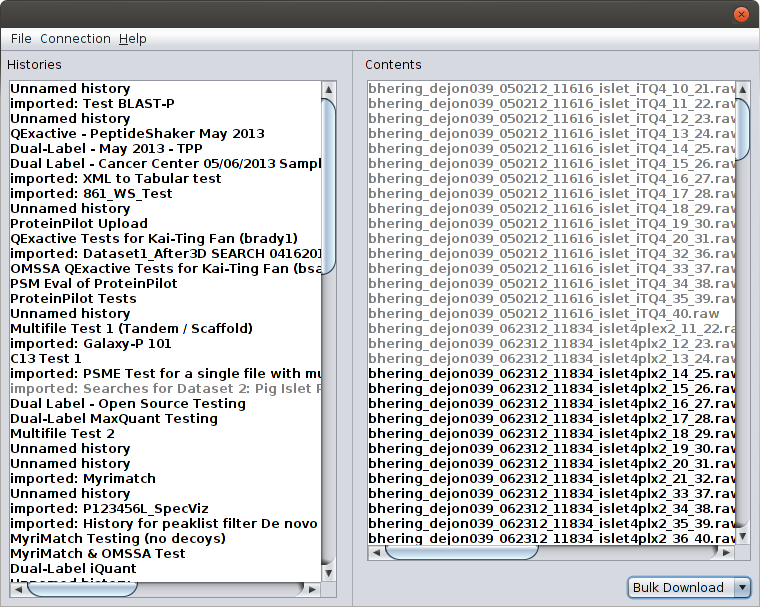
\includegraphics[scale=0.5]{bulkdownload_jgalaxy.png}
                              \end{figure}              
                            \end{column}
                          \end{columns}
                        \end{block}
                        \vfill
                        \begin{block}{Handling Large Numbers of Files - Tool Extensions}
                          \begin{columns}
                            \begin{column}{.2\textwidth}
                              \begin{figure}
                                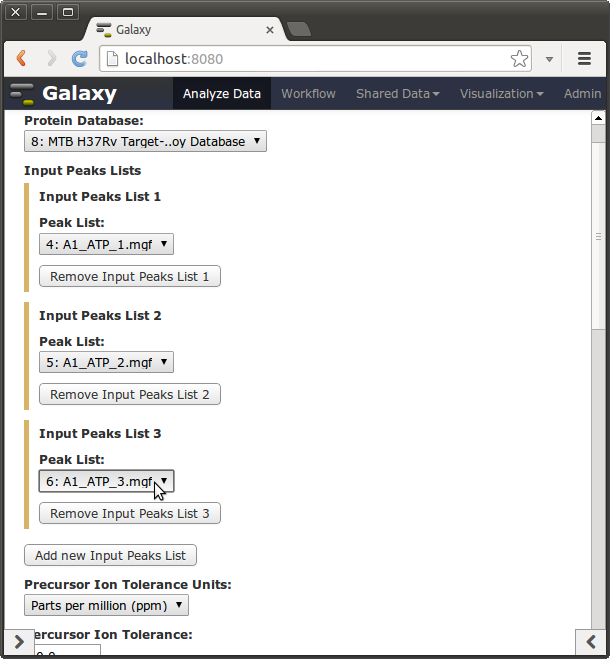
\includegraphics[scale=0.5]{mgf_select_repeat.png}
                                \caption{Traditional multiple input selection.}
                              \end{figure}
                            \end{column}
                            \begin{column}{.59\textwidth}
                            \begin{itemize}
                              \item Previously Galaxy required a lot of clicking and tracking to provide multiple inputs to a tool.
                              \item Our Galaxy tool extensions allow easy multiple selection.
                              \item Convenient for jobs requiring a few inputs, necessary for jobs requiring dozens or hundreds.
                              \item Used in many proteomics tools (e.g. MaxQuant, PeptideShaker, Scaffold, etc...).
                              \item Incorporated upstream in core Galaxy framework.
                            \end{itemize}
                            \end{column}
                            \begin{column}{.2\textwidth}
                              \begin{figure}
                                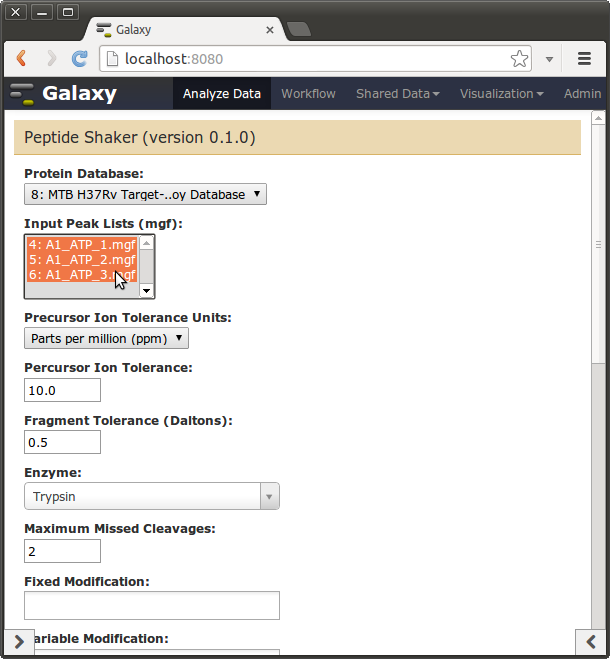
\includegraphics[scale=0.5]{mgf_select_multiple.png}
                                \caption{Our multiple input extension.}
                              \end{figure}              
                            \end{column}
                          \end{columns}            
                        \end{block}
                        \vfill
                      }
                    \end{minipage}
                  \end{beamercolorbox}
                \end{column}      
              \end{columns}
              \vfill
              \begin{block}{Handling Large Numbers of Files - Multiple File Datasets}
                \begin{columns}
                  \begin{column}{.30\textwidth}
                    \begin{figure}
                      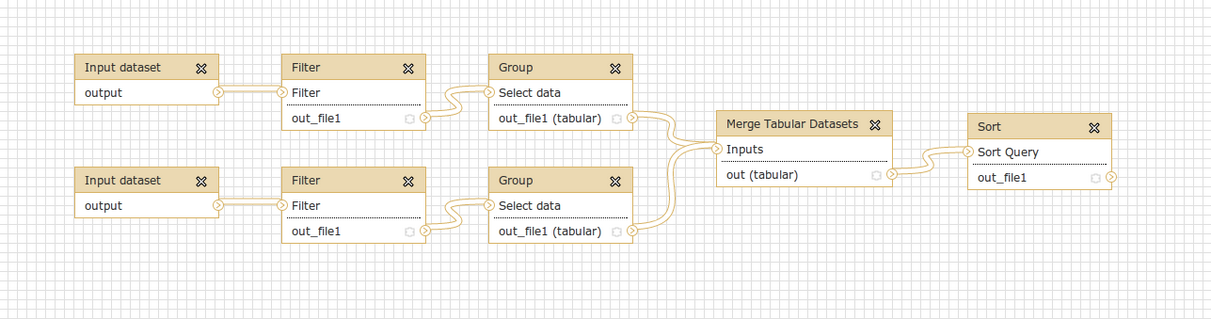
\includegraphics[scale=0.7]{workflow_two_inputs_cropped.png}
                      \caption{Traditional Galaxy workflows would not allow this workflow for two inputs to be used with three inputs.}
                    \end{figure}              
                    \vfill
                    \begin{figure}
                      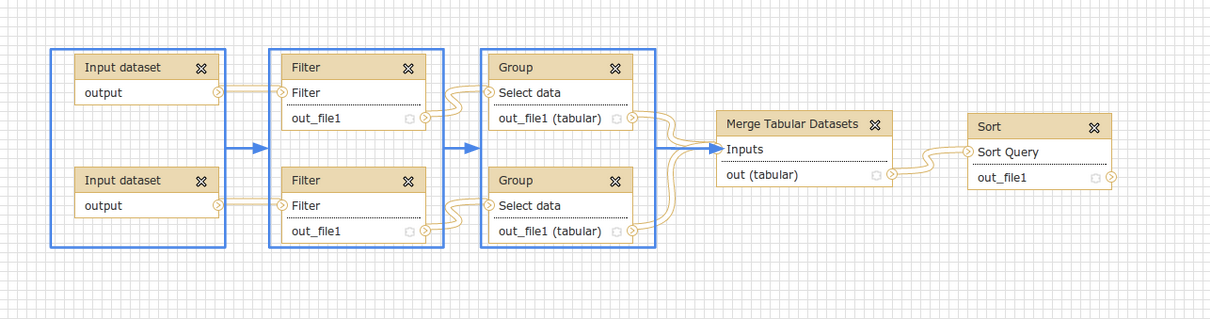
\includegraphics[scale=0.7]{workflow_two_input_combined_cropped.png}
                      \caption{Key innovation here it to group multiple files into a single dataset resulting in a flatter workflow.}
                    \end{figure}
                  \end{column}

                  \begin{column}{.43\textwidth}
                    Galaxy cannot create reusable workflows with variable number of input datasets. We have created the concept of multiple file datasets to address this deficiency.
                    \begin{itemize}
                      \item Key Idea: Group any number of files into one Galaxy "dataset". 
                      \item This allows workflows to act
                      \item Built on the Adapt (https://bitbucket.org/glormph/adapt), but extending the Galaxy framework to address this allows it to work with all tools and all datatypes.
                      \item Available as part of the galaxy-extras project (https://bitbucket.org/msiappdev/galaxy-extras).
                    \end{itemize}
                  \end{column}

                  \begin{column}{.25\textwidth}
                    \begin{figure}
                      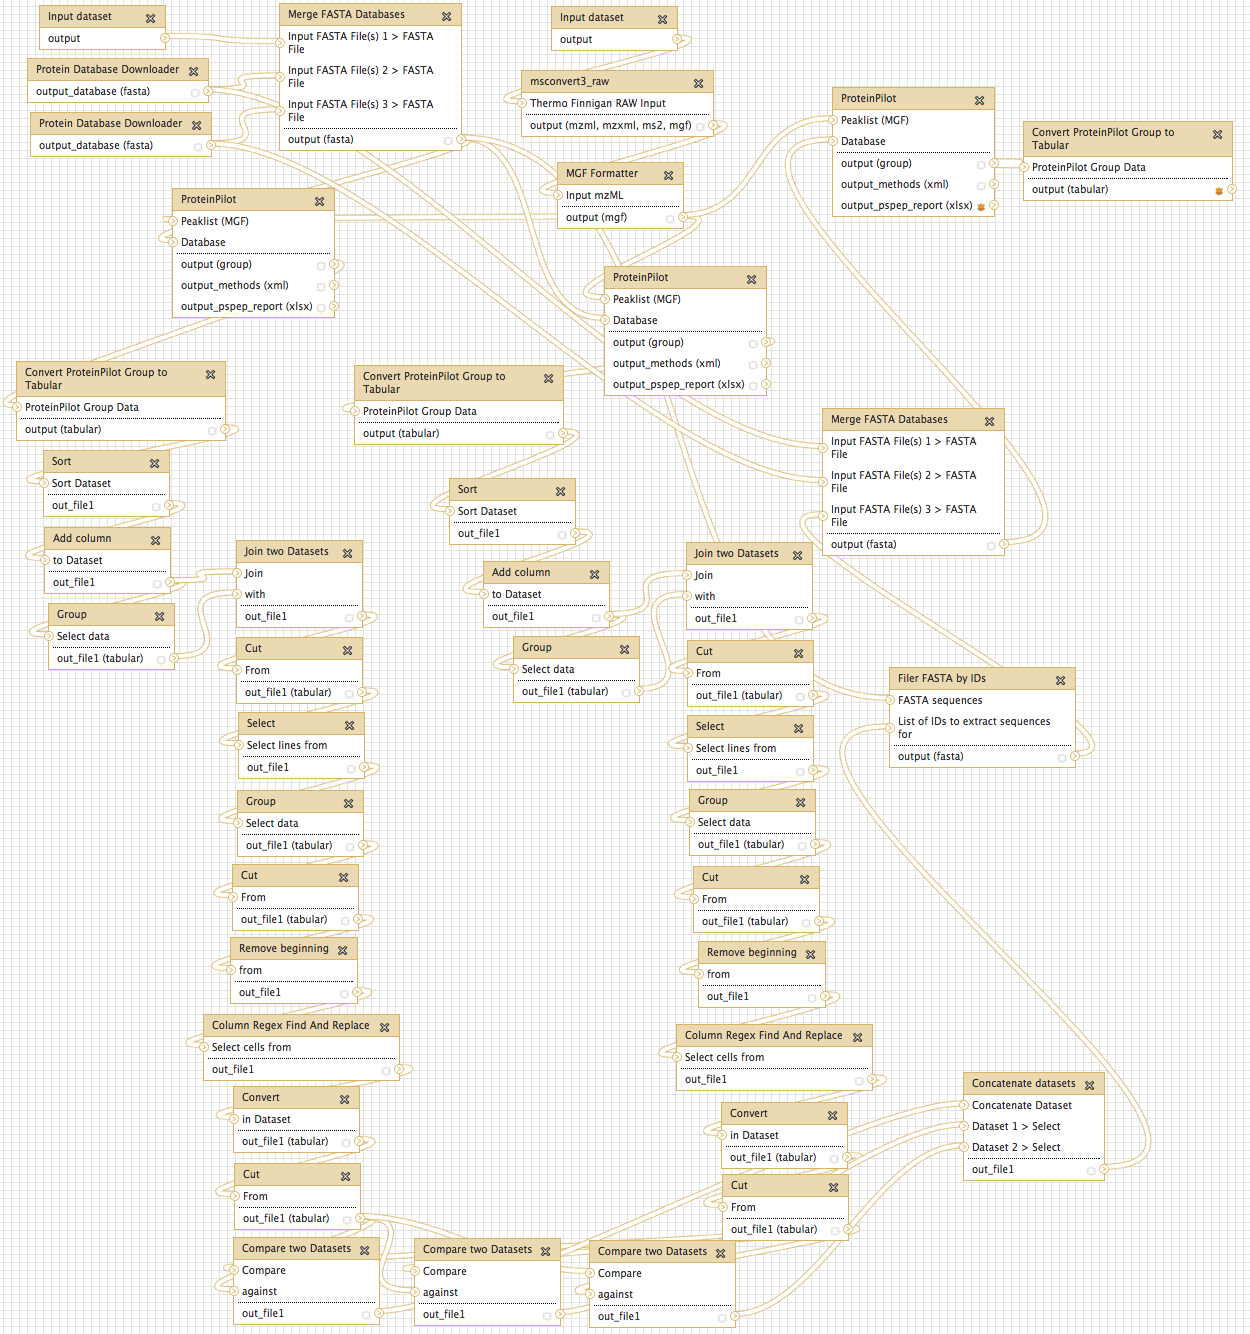
\includegraphics[scale=0.7]{minnesota_two_step.png}
                      \caption{This "Minnesota Two Step" workflow can operate over any number of peak lists, this is not possible in Galaxy without multiple file dataset extensions.}
                    \end{figure}              
                  \end{column}

                \end{columns}
              \end{block}
            }
          \end{minipage}
        \end{beamercolorbox}
      \end{column}              

      \begin{column}{.33\textwidth}
        \begin{beamercolorbox}[center,wd=\textwidth]{postercolumn}
          \begin{minipage}[T]{.98\textwidth} % tweaks the width, makes a new \textwidth
            \parbox[t][\columnheight]{\textwidth}{
              \begin{block}{Cross Platform Job Execution - Challenges}

              Perhaps driven by proprietary data formats, proteomics has a
              Windows-centric culture not present in genomics. As an upshot,
              previously there was no easy way to run Windows applications in
              the Galaxy framework.

              {\large\textsl
              The large number of important proteomics applications tied to the
              Windows platform nesseciatated the creation of the LWR.}


              \end{block}
              \vfill
              \begin{block}{Cross Platform Job Execution with the LWR}

              The LWR is an application that can be installed on any server
              (Windows or *nix) and allows a remote Galaxy instance to submit
              jobs to that host.

              \begin{itemize}
              \item https://lwr.readthedocs.org - Read more about installing the LWR and configuring Galaxy clients 
              \item https://bit.ly/galaxy-lwr-code - Check out the LWR source code.
              \end{itemize}

              \end{block}
              \vfill
              \begin{block}{Cross Platform Tool - msconvert}
                \begin{columns}
                  \begin{column}{.39\textwidth}
                    \begin{figure}
                      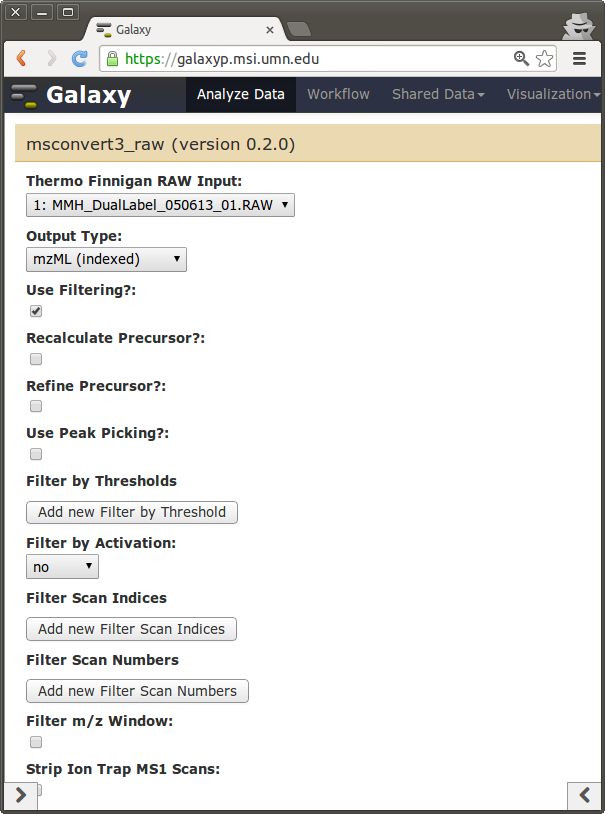
\includegraphics[scale=0.5]{msconvert3_screenshot.png}
                    \end{figure}              
                  \end{column}
                  \begin{column}{.60\textwidth}
                    \begin{itemize}
                      \item Describe MsConvert in Galaxy-P
                    \end{itemize}
                  \end{column}  
                \end{columns}            
              \end{block}
              \vfill
              \begin{block}{Cross Platform Tool - maxquant}
                \begin{columns}
                  \begin{column}{.60\textwidth}
                    \begin{itemize}
                      \item Describe MaxQuant in Galaxy-P
                    \end{itemize}
                  \end{column} 
                  \begin{column}{.39\textwidth}
                    \begin{figure}
                      \includegraphics[scale=0.5]{maxquant_screenshot.png}
                    \end{figure}              
                  \end{column}
                \end{columns}
              \end{block}
              \vfill
              \begin{block}{Cross Platform Tool - proteinpilot}
                \begin{columns}
                  \begin{column}{.39\textwidth}
                    \begin{figure}
                      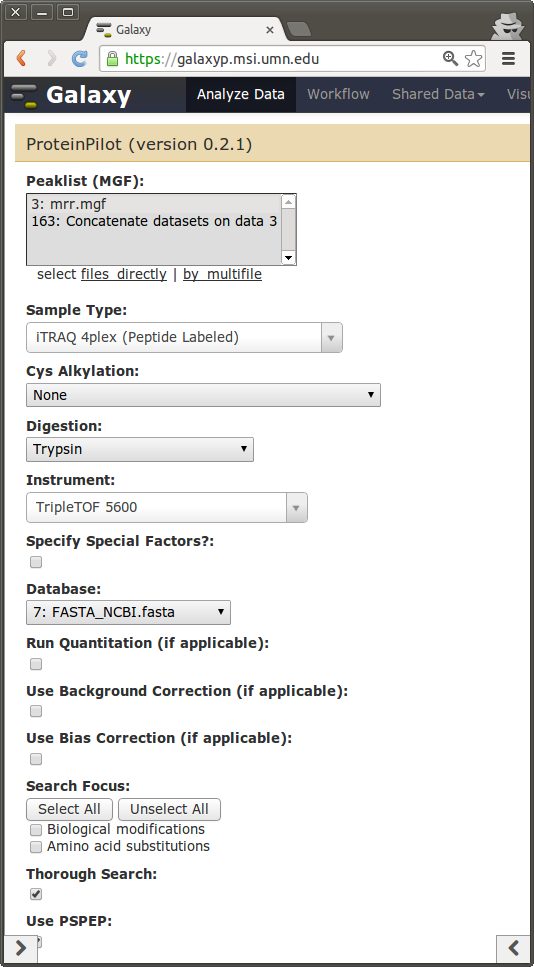
\includegraphics[scale=0.5]{proteinpilot_screenshot.png}
                    \end{figure}              
                  \end{column}

                  \begin{column}{.60\textwidth}
                    \begin{itemize}
                      \item Describe Protein Pilot in Galaxy-P
                    \end{itemize}
                  \end{column}              
                \end{columns}
              \end{block}
            }
          \end{minipage}
        \end{beamercolorbox}
      \end{column}              
    \end{columns}   
  \end{frame}
\end{document}
